\documentclass[12pt,twoside]{article}

% *** Set page dimensions ***
\raggedbottom
\parindent=0in
%\setlength{\topmargin}{-0.5in}
%\setlength{\oddsidemargin}{0.1875in}
%\setlength{\evensidemargin}{0in}
%\setlength{\textheight}{8.5in}
%\setlength{\textwidth}{6.225in}
%\addtolength{\oddsidemargin}{-0.7in}
%\addtolength{\evensidemargin}{-1.2in}
%\setlength{\oddsidemargin}{-0.2in}
%\setlength{\evensidemargin}{-0.2in}
%\addtolength{\textwidth}{1.4in}
%\addtolength{\topmargin}{-.875in}
%\addtolength{\textheight}{2.00in}

% *** Packages ***
\usepackage{alltt}
\usepackage{tocloft}
\usepackage{graphicx}
\usepackage{lscape}
\usepackage{amssymb}
\usepackage{float}
\usepackage{amsmath}
\usepackage{gensymb}
%\usepackage{subfigure}
\usepackage{lscape}
\usepackage{epsfig}
\usepackage{enumerate}
\usepackage{multicol}
\usepackage{fancyhdr}
\usepackage{epstopdf}
\usepackage{hyperref}
\usepackage{listings}

% *** Table of contents and Sectioning *** 
\setcounter{secnumdepth}{0}
\setcounter{tocdepth}{5}

% *** Table of contents and Sectioning *** 
\newcommand{\next}{\addtocounter{enumi}{9} \item}
\newcommand{\now}[1]{\setcounter{enumi}{#1}}
\newcommand{\Z}{\mbox{\sf Z\hspace{-1.5mm}Z}}
\newcommand{\R}{\mbox{\rm I\hspace{-0.75mm}R}}
\columnsep=0.75in

% *** Shortcuts for syntax ***
\newcommand{\ds}{\displaystyle }
\newcommand{\vsc}{\vspace{4mm}}
\newcommand{\dd}[1]{\frac{d}{d{#1}} \,} 
\newcommand{\ddx}{\frac{d}{dx} \,} 
\newcommand{\ddy}{\frac{d}{dy} \,} 
\newcommand{\ddz}{\frac{d}{dz} \,} 
\newcommand{\dydx}{\frac{dy}{dx} \,} 
\newcommand{\dydt}{\frac{dy}{dt} \,} 
\newcommand{\dfdx}{\frac{df}{dx} \,} 
\newcommand{\ddt}[1]{  \frac{d{#1}}{dt} }
\newcommand{\pp}[2]{  \frac{\partial{#1}}{\partial {#2}} }
\newcommand{\zx}{\frac{\partial z}{\partial x} \,}
\newcommand{\zy}{\frac{\partial z}{\partial y} \,}
\newcommand{\limh}{\lim_{h \rightarrow 0} \;}
\newcommand{\diff}{\frac{d}{dx} \,}
\newcommand{\de}{\Delta}
\renewcommand{\thesection}{\Roman{section}}
\newcommand{\bfr}{\begin{flushright}}
\newcommand{\efr}{\end{flushright}}
\newcommand{\dx}{\frac{\partial f}{\partial x} \,}
\newcommand{\dy}{\frac{\partial f}{\partial y} \,}
\newcommand{\p}{\partial}
\newcommand{\vi}{\vec{i}}
\newcommand{\vj}{\vec{j}}
\newcommand{\vk}{\vec{k}}
\newcommand{\lan}{\left\langle}
\newcommand{\ran}{\right\rangle}
\newcommand{\reading}[1] { {\em Reading: #1}}
\renewcommand{\Pr}{ \mbox{Pr}}

% *** Commands related to textbook references
\newcommand{\problem}{{\bf Problem.} }

% *** Footnoting with symbols ***
\long\def\symbolfootnote[#1]#2{\begingroup%
\def\thefootnote{\fnsymbol{footnote}}\footnote[#1]{#2}\endgroup}

% *** Defining a boxed note ***
\floatstyle{boxed}
\newfloat{noteinbox}{htb}{loa}
\newenvironment{boxnote}{\begin{noteinbox}[H]}{\end{noteinbox}}

\newcommand{\Question}{ {\bf Question: }  }
\newcommand{\Example}[1]{ {\bf Example: } {\em #1} }
\newcommand{\ExampleCont}[1]{ {\em #1} }

% *** Define the boxed Week #/summary at the beginning/end of every chapter ***
\newcommand{\sectionbox}[1]{% 
\begin{tabular}{|p{6in}|}%
\hline%
\ \\ %
{\Large {\bf {#1}}}  \\%
\ \\%
\hline%
\end{tabular}}

% *** Shortcuts *** 
\newcommand\goals{\large {\bf {Goals:}}}
\newcommand\setfont{ }

% *** Week commands: overwritten in each notes file
\newcommand{\Week}{Null-InPreambleCommon}
\newcommand{\WeekTitle}{Null-InPreambleCommon}
\newcommand{\Course}{MNTC P04}
\newcommand{\SetNum}{1 }
\newcommand{\topic}[1]{
\newpage
\setcounter{page}{1}
\fancyhead[LE,RO]{#1 - \thepage}
}

% *** Setup Latex for the large version of the files ***
%\usepackage[landscape]{geometry}
\usepackage[letterpaper,landscape,hmargin={.8in,.8in},vmargin={1in,0.2in}]{geometry}

% Remove paragraph indents
\setlength{\parindent}{0pt}

% Spacing at the top for the header is too large by default
\setlength{\voffset}{-5ex}

% **** RENEW SCALING COMMANDS HERE ****
% *** Text in boxes ***
\renewenvironment{boxnote}{\begin{noteinbox}[H] \huge}{\end{noteinbox}} 

% *** Chapter lead in/summary boxes ***
\renewcommand{\sectionbox}[1]{% 
\begin{tabular}{|p{9.5in}|}%
\hline%
\ \\ %
{\huge {\bf {#1}}}  \\%
\ \\%
\hline%
\end{tabular}}

% *** 'Section'' commands, which are sometimes used for spacing
% From http://zoonek.free.fr/LaTeX/LaTeX_samples_section/0.html
\makeatletter
 \renewcommand\section{\@startsection {section}{1}{\z@}%
                                    {-3.5ex \@plus -1ex \@minus -.2ex}%
                                    {0.3ex \@plus.2ex}%
                                    {\setfont\bf}}

 \renewcommand\subsection{\@startsection {subsection}{1}{\z@}%
                                    {-3.5ex \@plus -1ex \@minus -.2ex}%
                                    {0.3ex \@plus.2ex}%
                                    {\setfont\bf}}

% *** 'Goals' should be larger in the overheads ***
\renewcommand\goals{\huge {\bf {Goals:}}}
\renewcommand\setfont{\huge }

\thispagestyle{empty}

\setfont 

\newcommand{\WeekTitleOne}{Derivatives - Foundations}
\newcommand{\WeekTitleTwo}{Derivatives - Linearization and Applications}
\newcommand{\WeekTitleThree}{Derivatives - Modeling}
\newcommand{\WeekTitleFour}{Integrals - Foundations}
\newcommand{\WeekTitleFive}{Integrals - Techniques}
\newcommand{\WeekTitleSix}{Integrals - Modeling}
\newcommand{\WeekTitleSeven}{Differential Equations - }
\newcommand{\WeekTitleEight}{Differential Equations - }
\newcommand{\WeekTitleNine}{Differential Equations - }
\newcommand{\WeekTitleTen}{Linear Algebra - }
\newcommand{\WeekTitleEleven}{Linear Algebra - }
\newcommand{\WeekTitleTwelve}{Linear Algebra - }



\begin{document}
\setfont
\pagestyle{fancy}
\renewcommand{\Week}{4 }
\renewcommand{\WeekTitle}{\WeekTitleFour }

\fancyhead[LE,RO]{Week \Week}  % default, usually only for first page
\fancyfoot{}
\sectionbox{Week \#\Week: \WeekTitle}


\vspace{5mm}
\goals
\begin{itemize}
\item Use the definite integral to model and find a solution to a
  posed area- or accumulation-related problem.
\item Scale and add definite integrals, describe the meaning of
  integral bounds and how to apply them.
\item Recognize an anti-derivative of a function.
\item Apply the theory of the Fundamental Theorem of Calculus to
  evaluate simple integrals.
\item Distinguish between definite and indefinite integrals and their
  meaning.
\end{itemize}

\vspace{5mm}




\topic{Integration} 
\subsection*{Integration} 
If we had to summarize the first three weeks of the course, we would
say that the focus was on {\bf differentiation}.

All differentiation problems ask the same basic question: {\bf At what
  rate does a process change}, and how does that rate of change relate
to other characteristics of the process?

The key observation was that {\bf at small scales, rates of change look linear}.

\newpage

In the next three weeks of the course we will study {\bf integration}.
Again, the analysis will be made possible by the observation that on a
very small scale all processes look linear.  This time, though, we
will use this fact to see how regarding a process as an {\bf
  accumulation} of infinitely many small linear steps allows us to
calculate the accumulated total, even when the rate of accumulation is
far from linear.  {\bf Integration is always in some way about finding
  the total at the end of a process of accumulation.}

\newpage


 \topic{Distance and Velocity}
 \subsection*{Distance and Velocity}

 Recall that if we measure distance $x$ as a function of time $t$, the
 velocity is determined by differentiating $x(t)$: 
 \begin{center}
{\bf Velocity} is the {\bf slope} on the {\bf position graph}.
 \end{center}

 But now suppose we begin with a {\bf graph of the velocity} with
 respect to time.  How can we determine what {\bf distance} will be
 traveled?  Does distance also ``appear'' in the velocity graph
 somehow?

\newpage

\problem 
 Consider the graph for the velocity of a particle shown below. 
\begin{center}
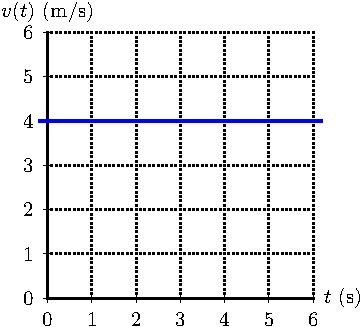
\includegraphics[width=0.25\linewidth]{graphics/notes_04_const_velocity}
\end{center}
How far did the particle travel between $t=0$ and $t=5$ seconds?
\begin{enumerate}[(a)]
\item 5 m\\[1ex]
\item 10 m\\[1ex]
\item 15 m\\[1ex]
\item 20 m
\end{enumerate}

\newpage
\problem 
~
\begin{center}
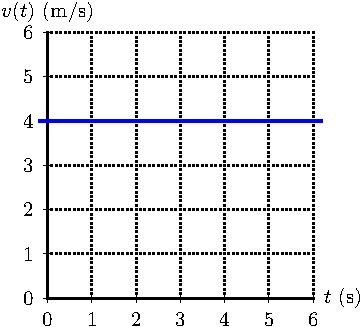
\includegraphics[width=0.25\linewidth]{graphics/notes_04_const_velocity}
\end{center}

Where does the distance traveled between $t=0$ and $t=5$ ``appear''
on this velocity graph?
\begin{enumerate}[(a)]
\item The distance traveled is the {\bf slope} between $t=0$ and $t=5$  \\[1ex]
\item The distance traveled is the {\bf average height} of the graph between $t=0$ and $t=5$  \\[1ex]
\item The distance traveled is the {\bf area} under the graph between $t=0$
  and $t=5$.
\end{enumerate}

\newpage

When the velocity is {\bf constant}, we have the equivalency:
\vspace{0.2in}
\begin{center}
dist = vel $\times$ time ~~~~ $\Longleftrightarrow$ dist = area under the velocity graph
\end{center}
\vspace{0.2in}

\problem 
What about when the velocity is {\bf not} constant though?

\begin{center}
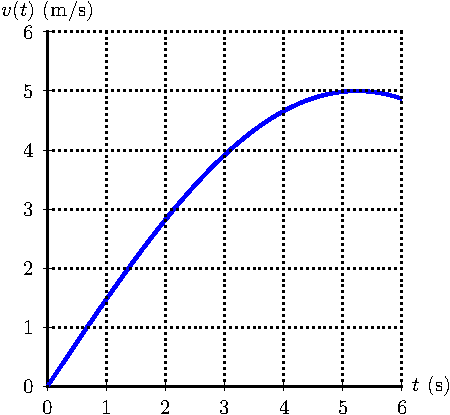
\includegraphics[width=0.35\linewidth]{graphics/notes_04_variable_velocity}
\end{center}

Do the units of the ``area'' under this graph still make sense as a
distance value?


\vfill
\newpage
\topic{Estimating Areas}
\subsection*{Estimating Areas}

It appears that
\begin{center}
{\bf distance traveled} = {\bf area under the graph of velocity}
\end{center}
even when the velocity is changing.  This means that we've found two
equivalent problems, and
can work with whichever version benefits us the most at a particular moment. \\


Unfortunately, many or most arbitrary areas are essentially impossible
to find when the shape isn't a composition of simple shapes (e.g. triangles, rectangles, or circles). \\[1ex]

In these cases, we must compute the area using less direct methods.
We will start by making an {\em estimate} of the area under the graph
using shapes whose area is easier to calculate.

\newpage

\problem Suppose we are trying to find the area underneath the graph of the
function $f(x)$ given below between $x = 1$ and $x=4$.  Shade in that
region, and call that area $A$.

\begin{center}
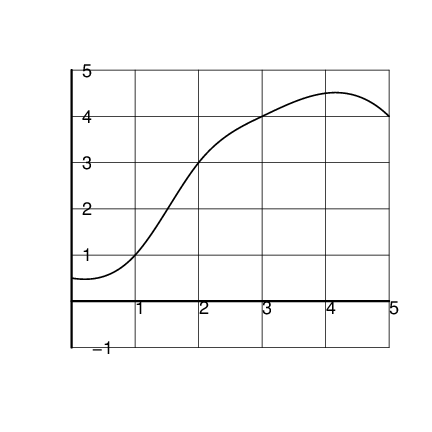
\includegraphics[width=4in]{graphics/notes_04_graph06}
\end{center}


\newpage
We can make a rough estimate of the area by drawing a rectangle that
completely contains the area, or a rectangle that is completely
contained by the area.


\problem 
{Calculate this overestimate and underestimate for the
  area $A$.}
  
\hfill 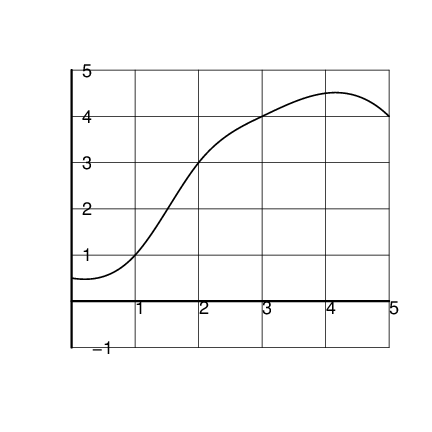
\includegraphics[width=4in]{graphics/notes_04_graph06}


\newpage The next step is to use smaller rectangles to improve our
estimate the area.  We can divide the interval from $x = 1$ to $x = 4$
into 3 intervals of width 1, and use different size rectangles on each
interval.



\problem Estimate the area $A$ by using 3 rectangles of width 1.
  Use the function value at the {\em left} edge of the interval as the
  height of each rectangle.

\hfill 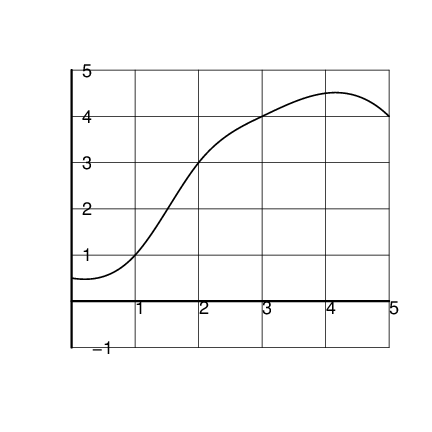
\includegraphics[width=0.43\linewidth]{graphics/notes_04_graph06}

\newpage

We can repeat this process for any number of rectangles, and we expect
that our estimation of the area will get better the more rectangles we
use.  The method we used above, choosing for the height of the
rectangles the function at the left edge, is called the {\bf left hand
  sum}, and is denoted $\mbox{LEFT}(n)$ if we use $n$ rectangles.

\newpage

\topic{Generalizing Area Calculation with Summation Notation}
\subsection*{Generalizing the Area Calculation}

Suppose we are trying to estimate the area under the function $f(x)$
from $x = a$ to $x = b$ via the left hand sum with $n$ rectangles.
\begin{itemize}
\item the {\bf width} of each rectangle will be $\Delta x =
\displaystyle\frac{b-a}{n}$.  
\item If we label the endpoints of the intervals to be
  $a = x_{0} < x_{1} < \cdots < x_{n-1} < x_{n} = b$, then the {\bf
    heights} of the rectangles will be $f(x_{i})$'s, and
\item the formula for the left hand sum/area will be
\end{itemize}

\begin{align*}
  \mbox{LEFT}(n) = & f(x_{0}) \Delta x+ 
 f(x_{1}) \Delta x + \ldots + 
 f(x_{n-1}) \Delta x 
\\  = & \displaystyle\sum_{i=1}^{n} f(x_{i-1})\Delta x.
\end{align*}

\newpage

\subsection*{Aside: Summation Notation}

The capital Greek letter sigma, $\sum$, is used as a short form notation for long sums.
E.g.
$$\ds \sum_{i=1}^n x_i$$

\newpage
\problem 
Translate the following into more traditional sums:

$\ds \sum_{i=1}^{100} i= $ \vfill 

$\ds \sum_{n=1}^{10} n^2 + n= $  \vfill

$\ds \sum_{i=1}^{n}  f(x_{i-1}) ~\Delta x= $
\vfill

\newpage 

Summation notation lends itself very nicely to translations between
hand-written sums and MATLAB computations.  A \texttt{for} loop can be
mapped easily on to a sum.

\problem Implement each of the sums below as a MATLAB loop and compute
the total. \\

$\ds \sum_{i=1}^{100} i= $ \vfill 

$\ds \sum_{n=1}^{10} n^2 + n= $  \vfill

\newpage


\topic{Riemann Sums}
\subsection*{Riemann Sums}

Area estimations like $\mbox{LEFT}(n)$ are examples of {\bf Riemann sums},
after the mathematician Bernhard Riemann (1826-1866) who formalized
many of the techniques of calculus.  The general form for a Riemann
Sum is

\begin{align*}
 f(x_{1}^{*}) \Delta x+ f(x_{2}^{*}) \Delta x + \ldots + f(x_{n}^{*}) \Delta x 
 \\ = \displaystyle\sum_{i=1}^{n} f(x_{i}^{*})\Delta x
\end{align*}

where each $x_{i}^{*}$ is some point in the interval $[x_{i-1},
x_{i}]$.  For $\mbox{LEFT}(n)$, we choose the left hand endpoint of the
interval, so $x_{i}^* = x_{i-1}$.

\newpage

The common property of all these
approximations is that they involve
\begin{itemize}
\item a sum of rectangular areas, with \\[1ex]
\item widths ($\Delta x$), and \\[1ex]
\item heights ($f(x_i^*)$)
\end{itemize}

There are other Riemann Sums that give slightly better estimates of
the area underneath a graph, but they often require extra computation.

\newpage


We observed that as we increase the number of rectangles used to
approximate the area under a curve, our estimate of the area under the
graph becomes more accurate.  We can see that based on an example like
the graph below:

\begin{center}
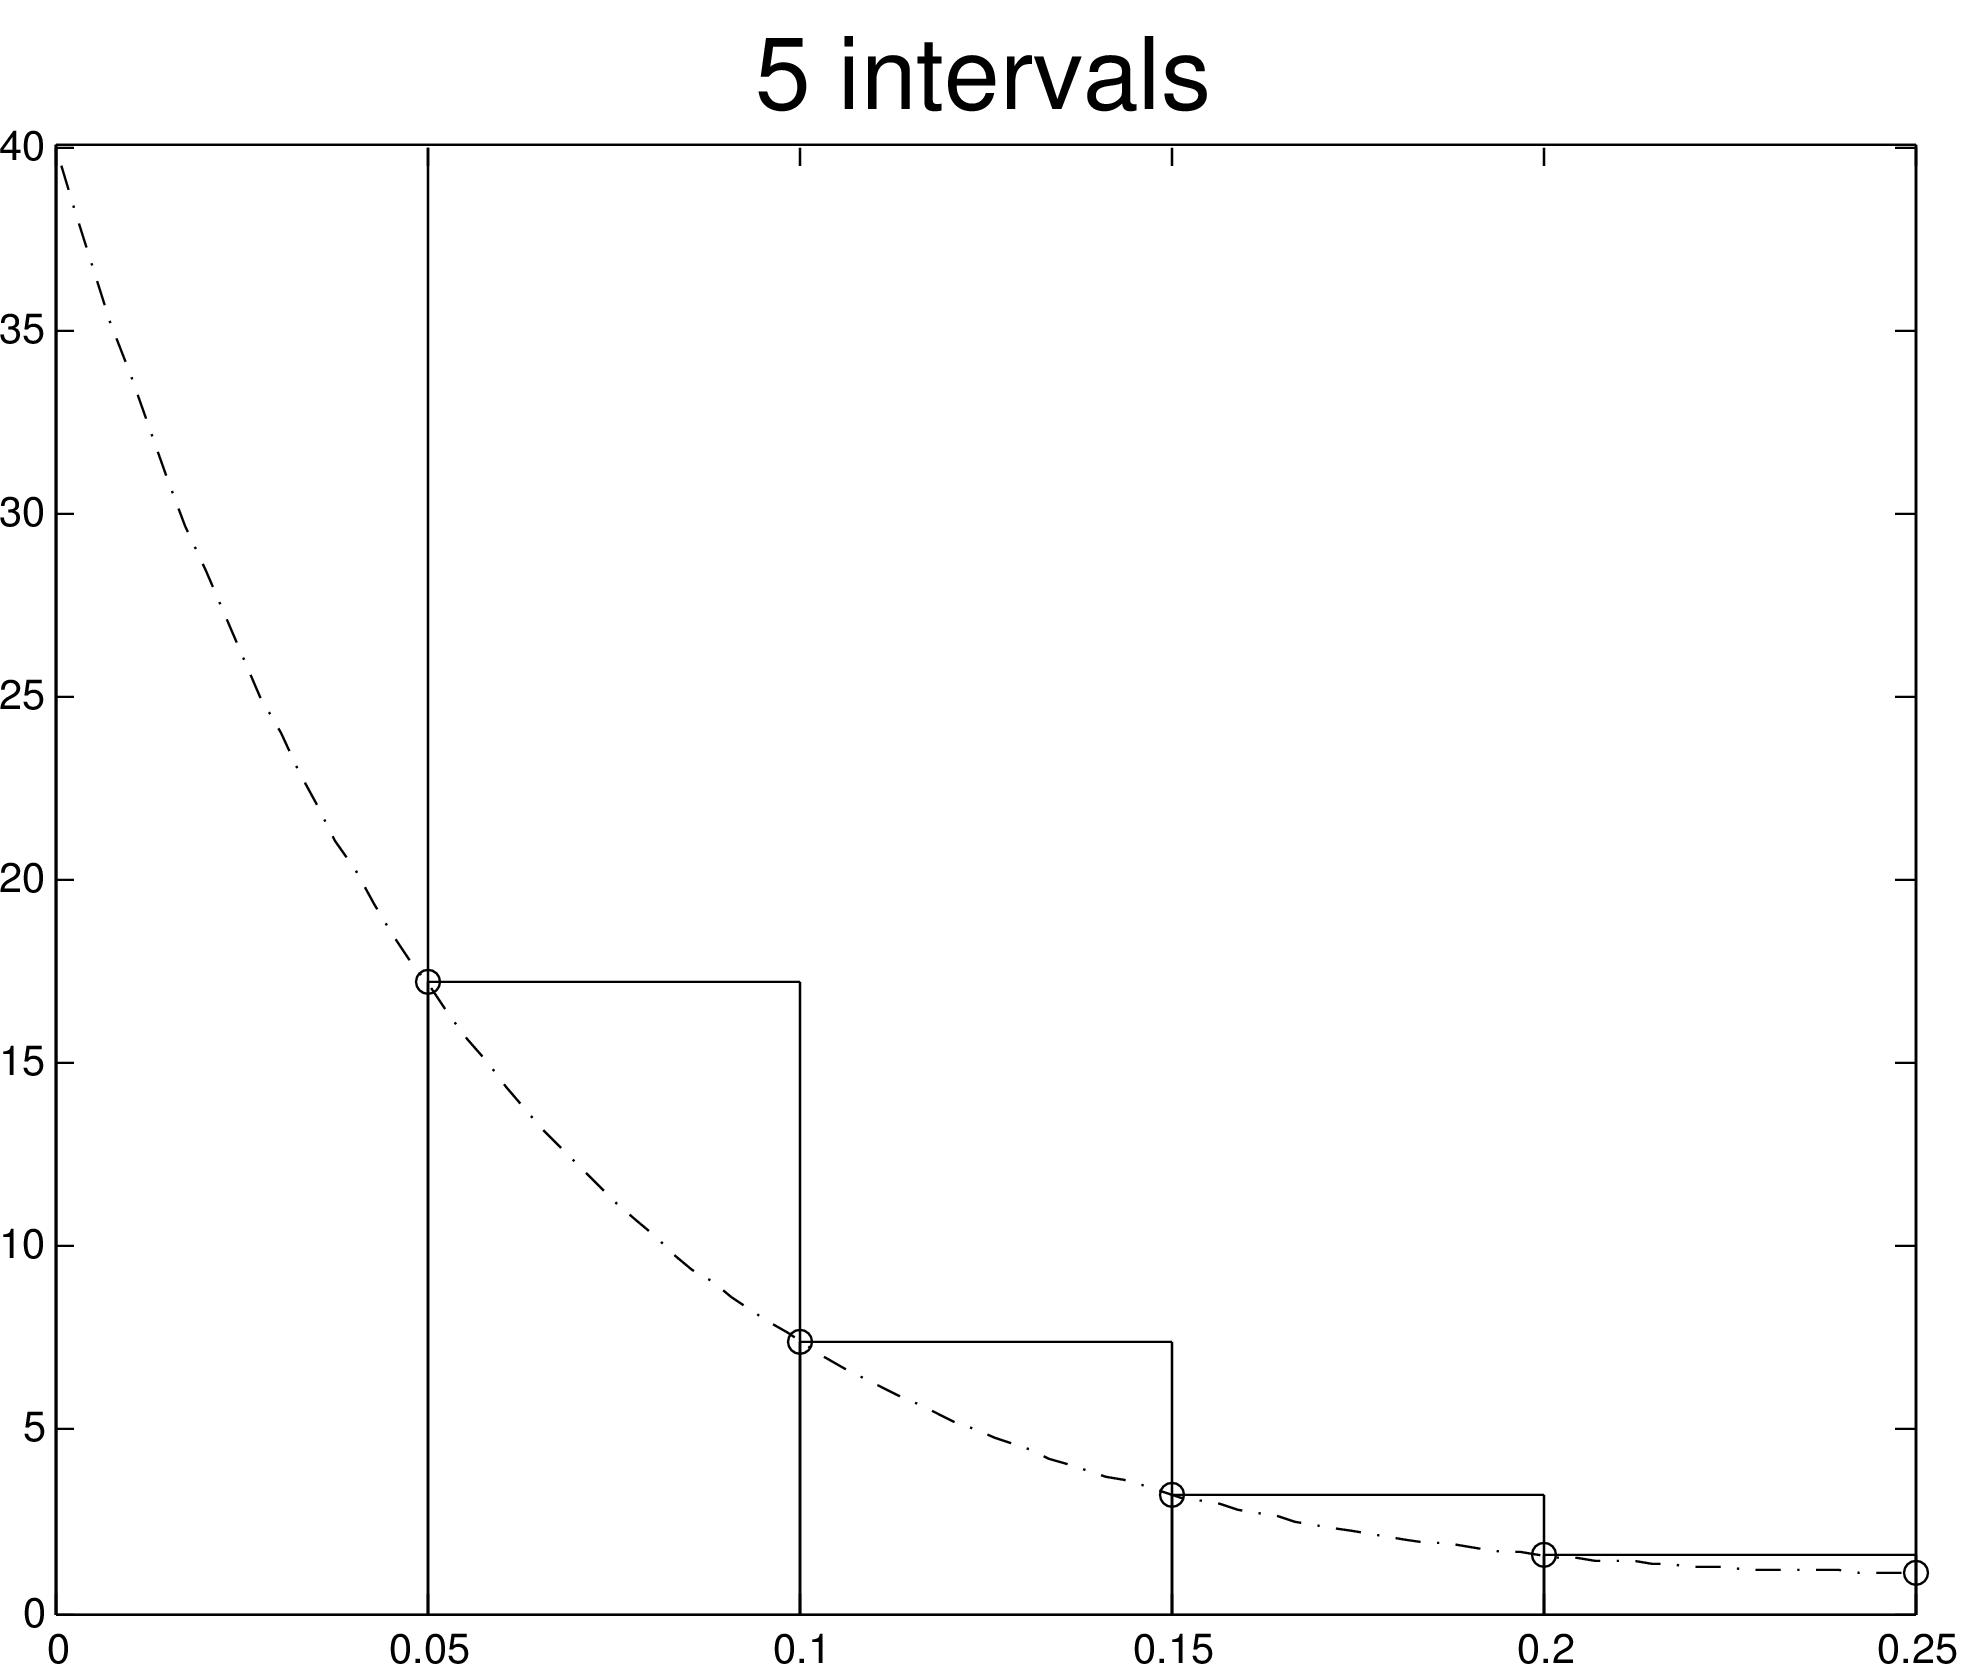
\includegraphics[height=4.5cm]{graphics/notes_04_f_lhr_5_intervals}
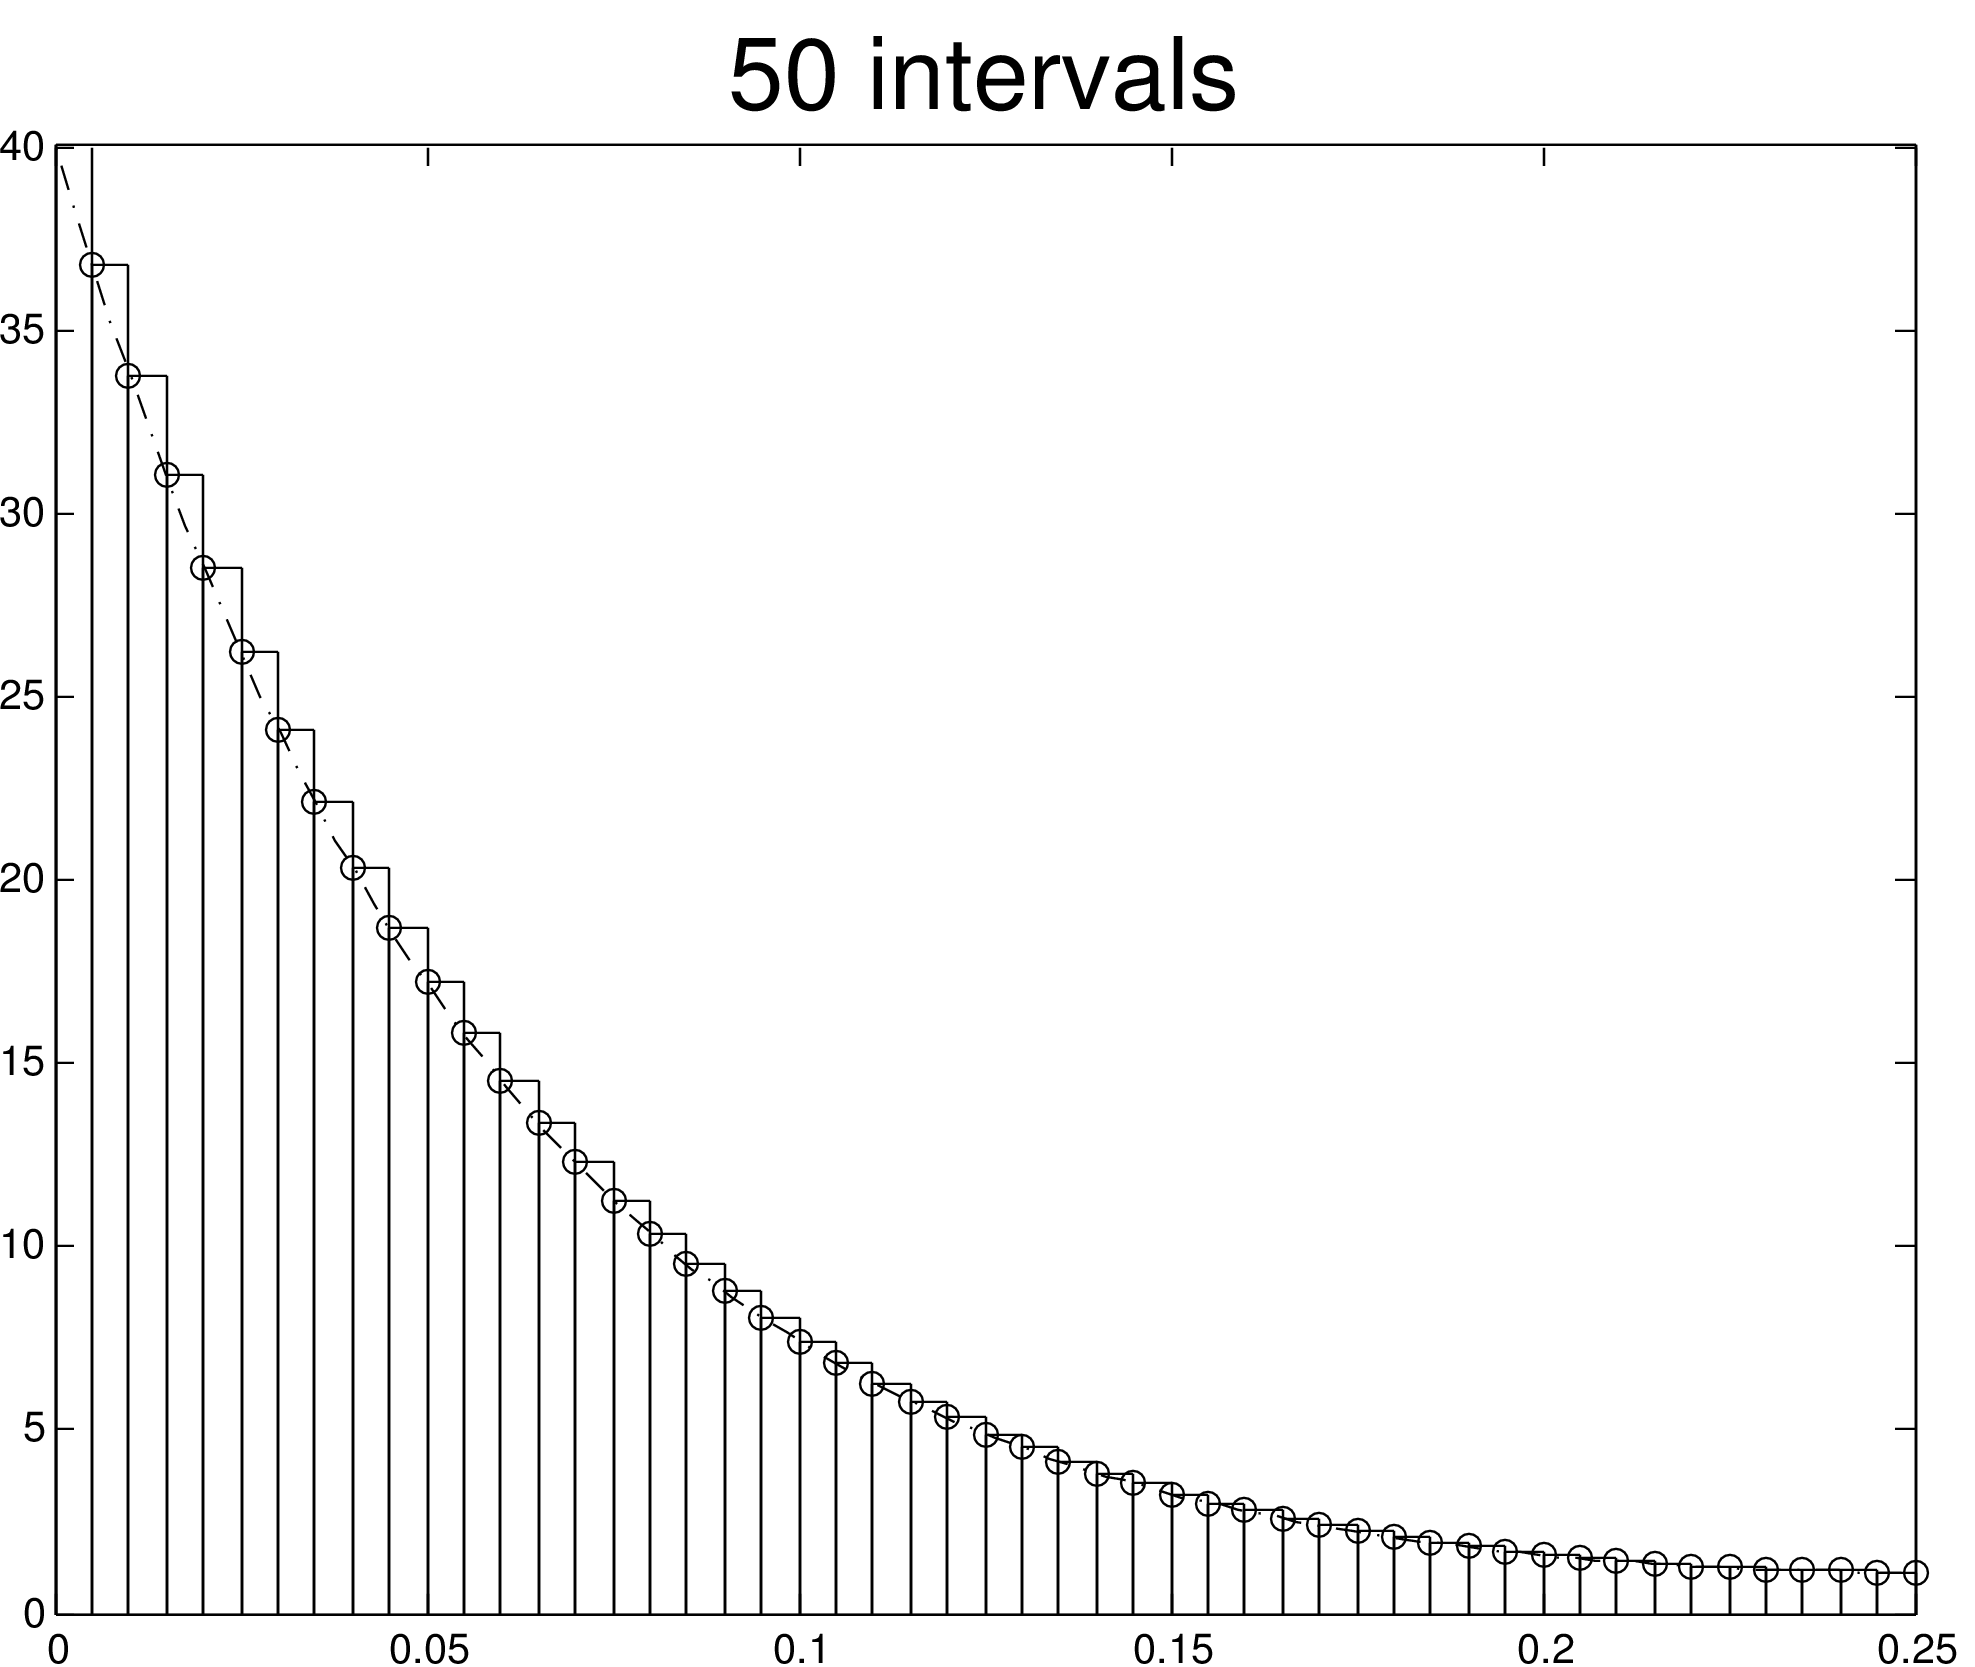
\includegraphics[height=4.5cm]{graphics/notes_04_f_lhr_50_intervals}
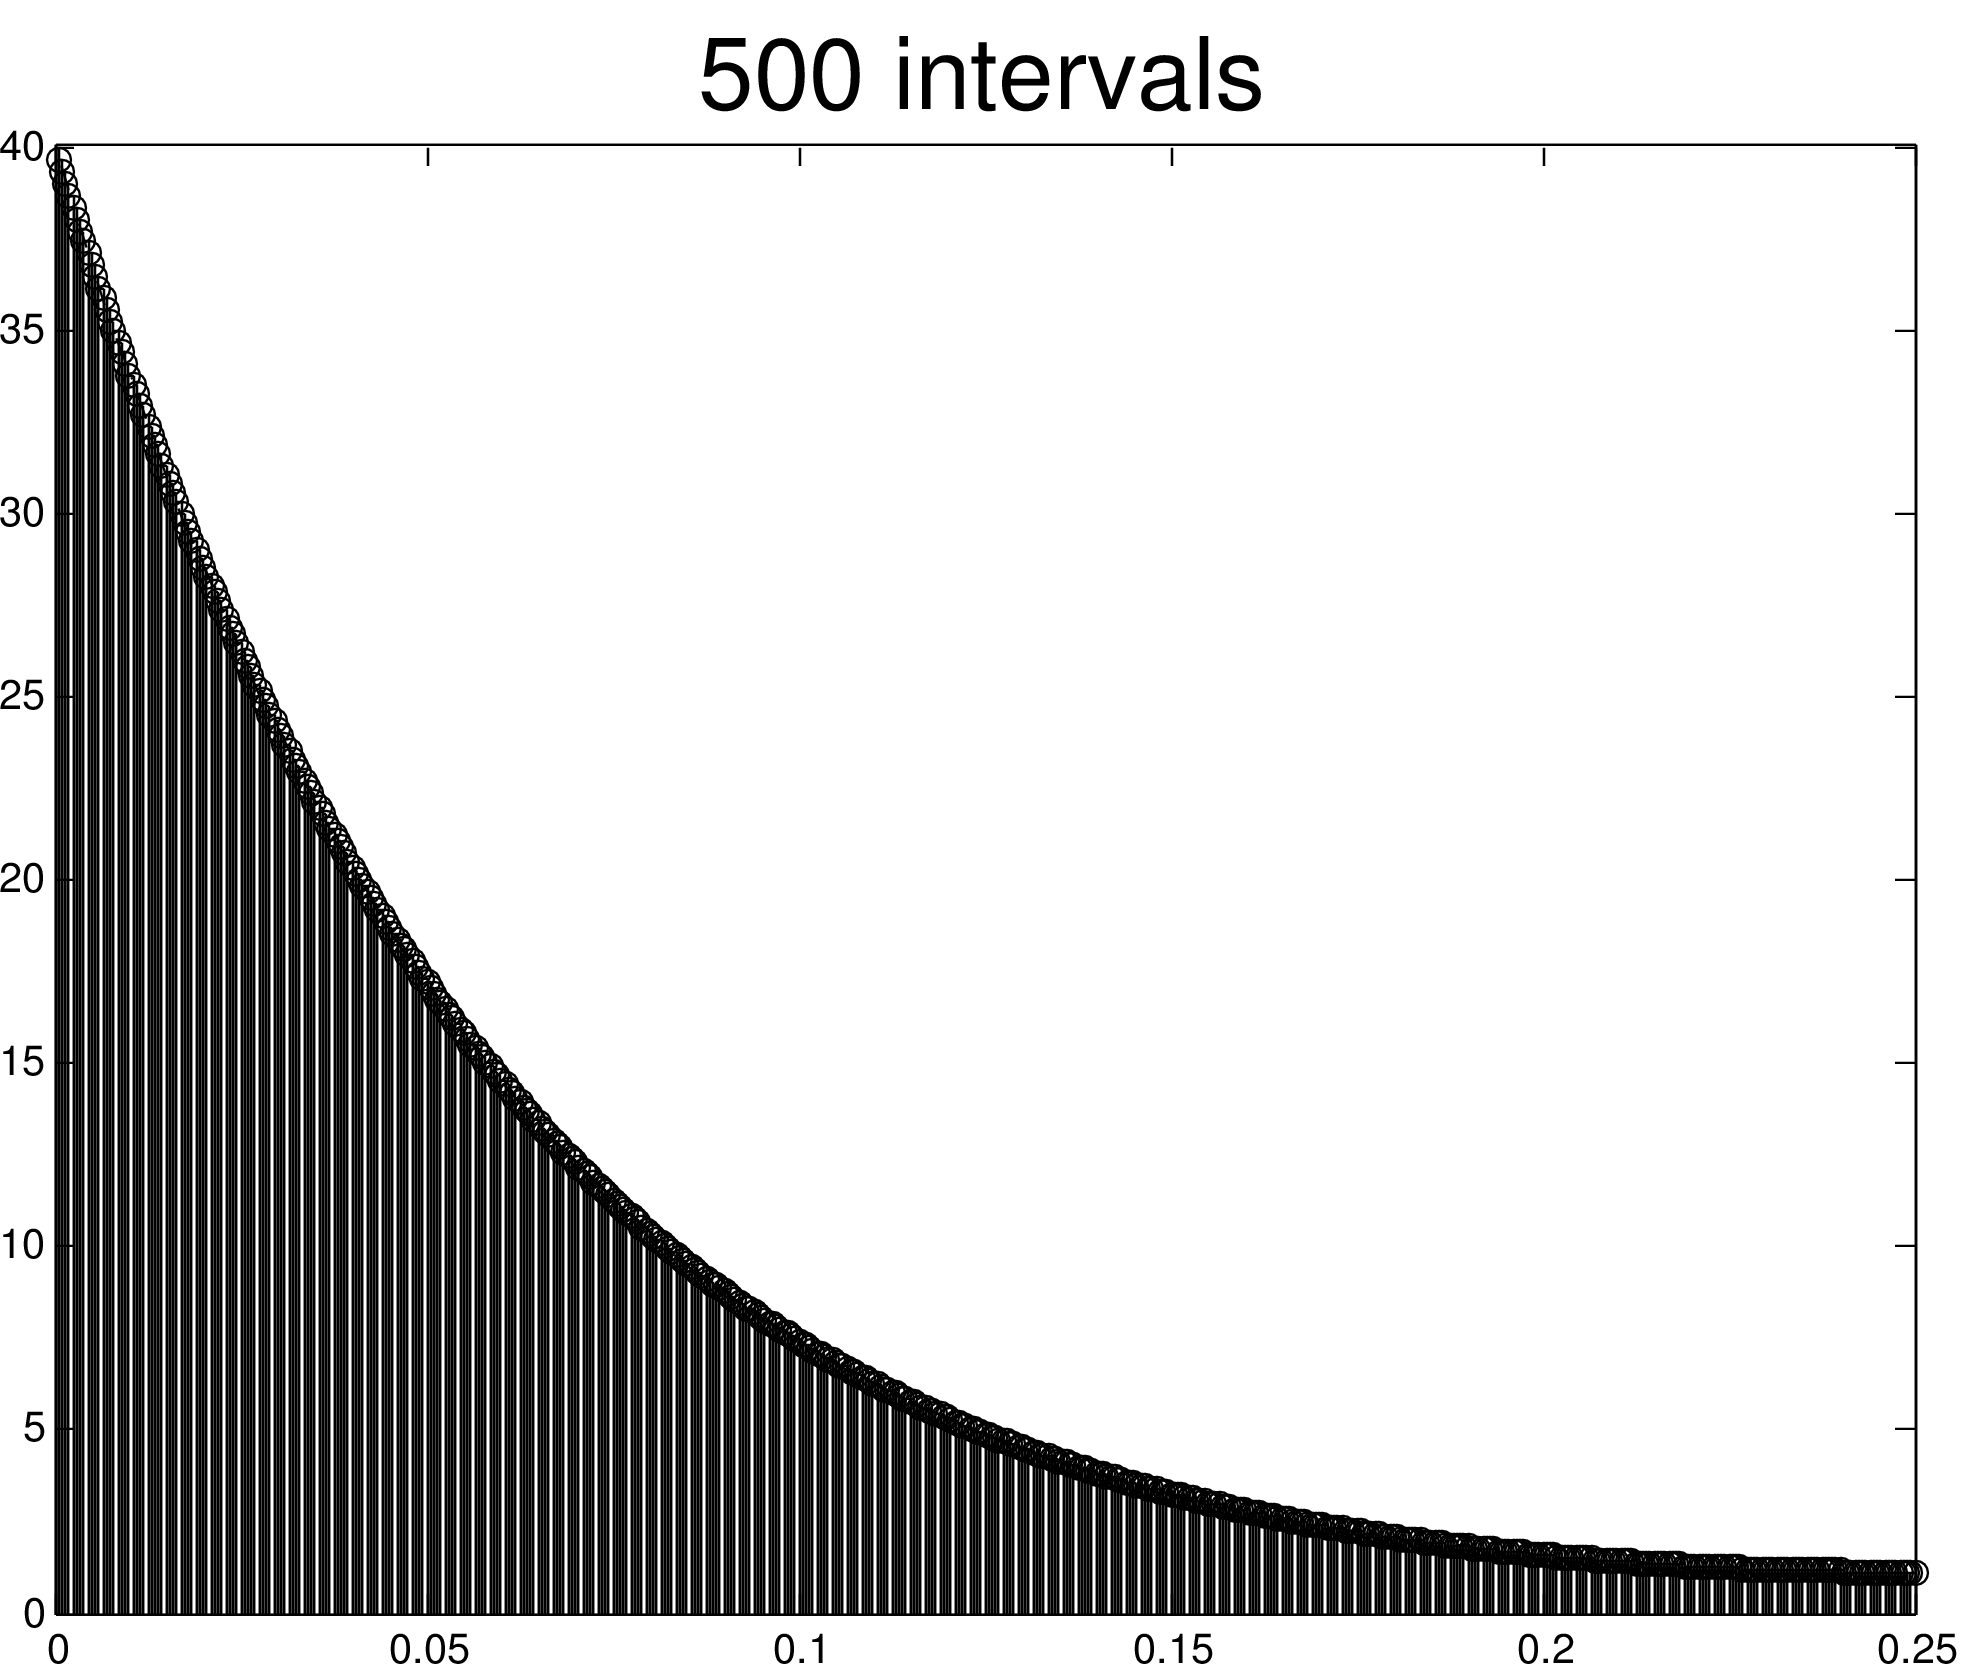
\includegraphics[height=4.5cm]{graphics/notes_04_f_lhr_500_intervals}
\end{center}

This implies that to obtain the {\bf
  exact area}, we should use a {\bf limit} on our Riemann sums.

\medskip
\begin{center}
The area underneath the graph of $f(x)$ between $x=a$ and $x=b$ is equal to $\displaystyle\lim_{n \to \infty} \mbox{LEFT}(n) = 
\displaystyle\lim_{n \to \infty} \displaystyle\sum_{i=1}^{n} f(x_{i-1})\Delta x$, ~~~where $\Delta x = \displaystyle\frac{b-a}{n}$.
\end{center}

\newpage

This limit, which gives the {\bf exact value of the accumulation of
  $f(x)$} is called the {\bf definite integral} of $f(x)$ from $a$ to
$b$, and is equal to the area under curve whenever $f(x)$ is a
non-negative continuous function.

\newpage
\topic{The Definite Integral}
\subsection*{The Definite Integral}

  
  The definite integral of $f(x)$ between $x=a$ and $x=b$ is denoted
  by the symbol
  $$\int_a^b f(x) \,dx ~~~~= \lim_{n \to \infty}
  \displaystyle\sum_{i=1}^{n} f(x_{i-1})\Delta x$$

We call $a$ and $b$ the
  {\bf{limits of integration}} and $f(x)$ the {\bf{integrand}}.  Note
  that this notation shares the same common structure with Riemann
  sums:
\begin{itemize}
\item a sum ($\ds \int $ sign) \\
\item widths ($dx$), and \\
\item heights ($f(x)$)
\end{itemize}

\newpage 

\problem Write the definite integral representing the area underneath
  the graph of $f(x) = x + \cos x$ between $x=2$ and $x=4$.

\vfill

\newpage
\problem Write an integral that represents the area under the graph of
$f(x) = x^2$ on the interval $x \in [0, 2]$.

\vfill \problem Sketch how the LEFT(4) estimate would be represented
graphically, and how it differs from the integral value.

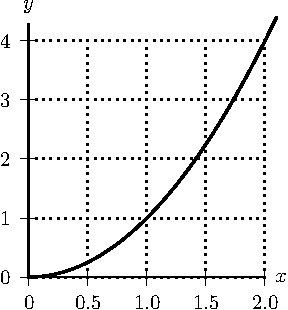
\includegraphics[width=0.3\linewidth]{graphics/notes_04_parabola_for_areas}
\hfill
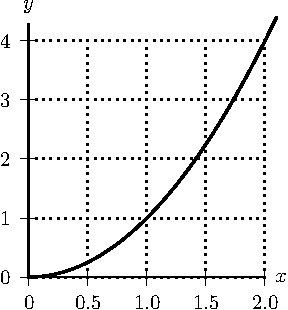
\includegraphics[width=0.3\linewidth]{graphics/notes_04_parabola_for_areas}


\newpage
\problem Use a LEFT sum with $n=4$ to estimate
$\displaystyle \int_{0}^{2}x^2\,dx$.

\vfill
\vfill

Repeat your LEFT estimate, but using MATLAB.

\vfill Repeat the calculation again in MATLAB, but now with 100
intervals.

\vfill

\newpage
Students often ask why instructors discuss Riemann sums, if they just
lead to definite integrals.

\begin{boxnote}
{\bf The Role of Riemann sums}
\begin{enumerate}
\item They are needed to say what we mean by an integral. \\[2ex]
\item They enable us to decide which integral is appropriate in a word
problem. \\[2ex]
\item They can also be used, with a finite number of intervals, to
  give an approximate value of the integral. \\[1ex]
\end{enumerate}
\end{boxnote}

\vspace{0.5in}

\topic{Negative Integral Values}
\subsection*{Negative Integral Values}

So far we have only dealt with the areas under/integrals of {\bf
  positive} functions.  Will the definite integral still be equal to
the area underneath the graph if $f(x)$ is always negative?  What
happens if $f(x)$ crosses the $x$-axis several times?



\problem Suppose that $f(x)$ has the graph shown below, and that A, B,
  C, D, and E are the areas of the regions shown.

\begin{center}
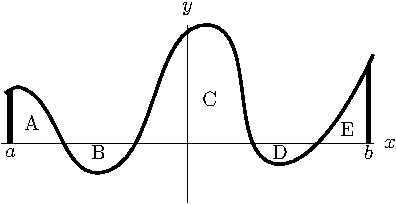
\includegraphics[width=0.6\linewidth]{graphics/notes_04_negative_area_example}
\end{center}

\newpage
\begin{center}
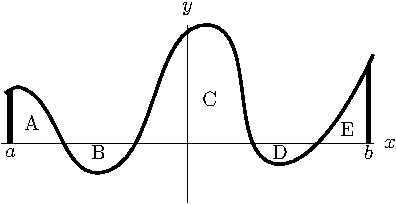
\includegraphics[width=0.4\linewidth]{graphics/notes_04_negative_area_example}
\end{center}

If we were to partition $[a,b]$ into small subintervals and construct a corresponding Riemann sum, then the first few terms in the Riemann sum would correspond to the region with area A, the next few to B, etc. 

\problem 
Which of these sets of terms have positive values?

\vfill

Which of these sets have negative values?
\vfill

\newpage

\begin{center}
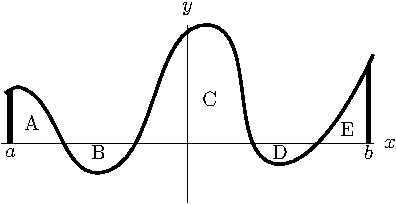
\includegraphics[width=0.3\linewidth]{graphics/notes_04_negative_area_example}
\end{center}
\problem 
{Express the integral $\displaystyle \int_a^b f(x) dx$ in
  terms of the (positive) areas A, B, C, D, and E.  }

\vfill
\vfill

{If $f$ were to represent velocity over time, what would the ``negative
  areas'' represent?}

\vfill
\newpage

\topic{The Fundamental Theorem of Calculus}
\subsection*{The Fundamental Theorem of Calculus}
We started our discussion of integration by stressing
the fact that an integral problem is always at heart a problem in
which something {\bf accumulates}. 

We then converted that accumulation problem into the problem of
computing the {\bf area under a graph}, and representing 
both using the notation

$$\ds \int_a^b f(x)~dx.$$

So far, we don't know how to evaluate that exactly: we can only use our approximation
based on a Riemann Sum,
$$\ds \int_a^b f(x)~dx \approx \sum_{i=1}^n f(x_i*) ~dx$$

If we want to evaluate this integral exactly, we need a new tool.

\newpage

The new idea is one of the most important discoveries in calculus: the
connection between integrals and the {\bf inverse of
  differentiation}. \\[1ex]

\begin{boxnote} ~\\ 
{\bf Fundamental Theorem of Calculus} \\

If $f$ is continuous and $F$ is an {\bf anti-derivative} of $f$, then 
\[ \int_a^b f(x)\,dx=F(b)-F(a).
\] 
\end{boxnote}

\problem Explain in words how we would use this to evaluate an
integral over the interval $x =a \ldots b$.

\vfill

\newpage

\subsection*{Using the Fundamental Theorem of Calculus}
To use the Fundamental Theorem of Calculus, we need to know formulas
for the anti-derivatives of functions.  We already know quite a few.

\newpage

\problem
Complete the following table of basic anti-derivatives by
asking yourself the question, ``$f(x)$ is the derivative of what
function, $F(x)$?''.

\begin{center}
\fbox{\begin{tabular}{cp{0.5in}c} 
{\bf Function $f(x)$} & & {\bf Anti-derivative $F(x)$}\\[0.25cm]
$x^n$ ($n \neq -1$) &  \\[0.5cm]
$\displaystyle \frac{1}{x}$ & \\[0.5cm]
$e^x$ & \\[0.5cm]
$\cos x$ & \\[0.5cm]
$\sin x$ & \\[0.5cm]
$\sec^2 x$ & \\[0.5cm]
$\displaystyle \frac{1}{\sqrt{1-x^2}}$ & \\[0.5cm]
$\displaystyle \frac{1}{1+x^2}$ & \\[0.5cm]
\end{tabular}}
\end{center}

\newpage
\topic{Fundamental Theorem - Simple Examples}
\subsection*{Fundamental Theorem - Simple Examples}

\problem Use the Fundamental Theorem to calculate the area under one
section of the graph of $\sin x$, the part from 0 to $\pi$.
\begin{center}
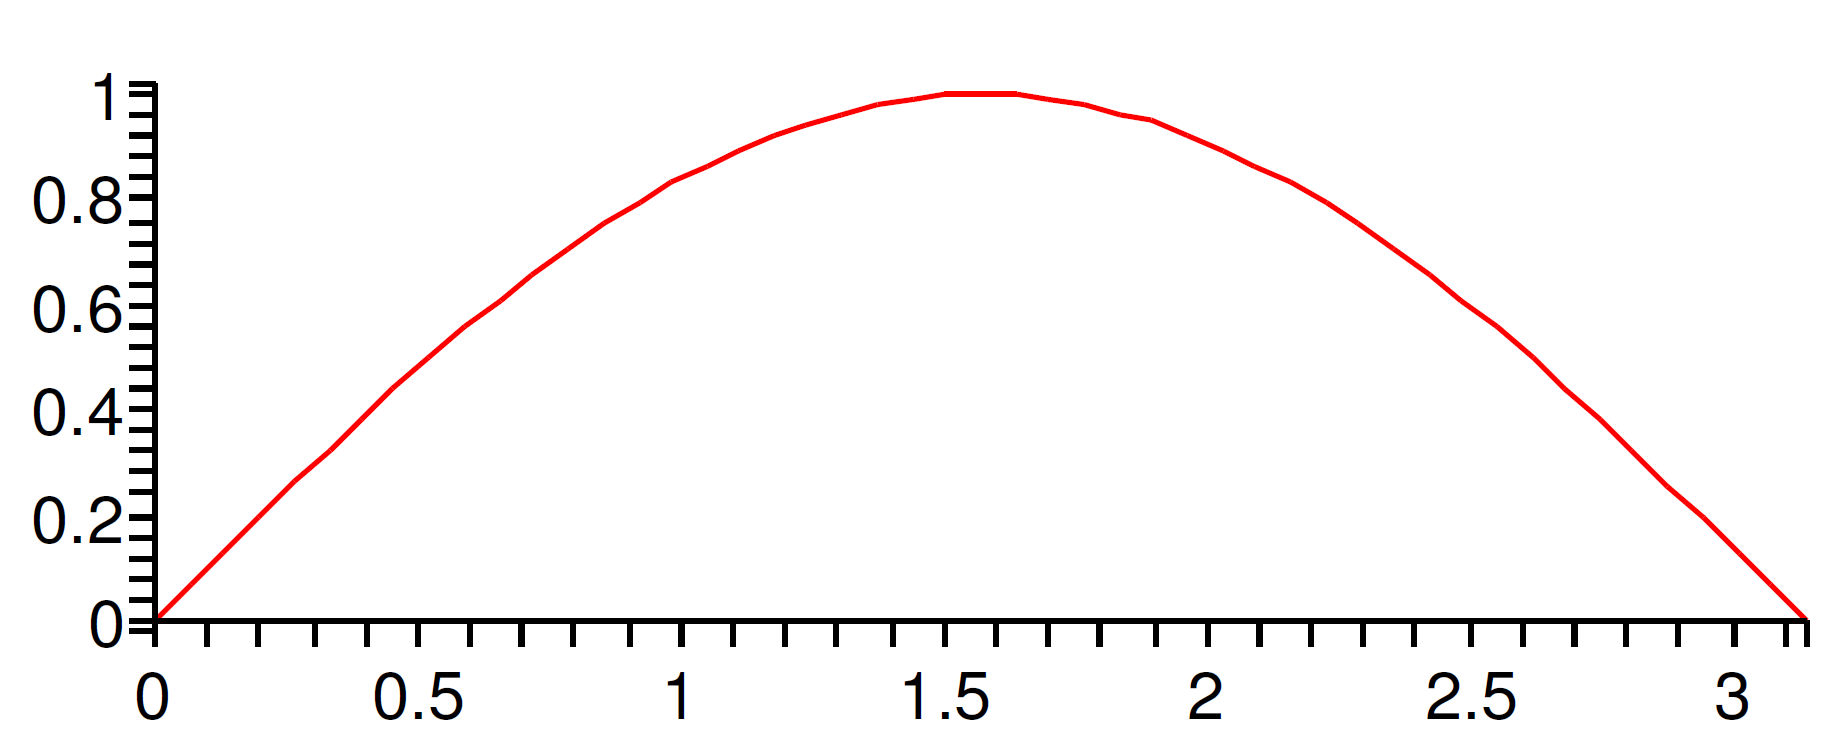
\includegraphics[width=7.5cm]{graphics/notes_04_sin}
\end{center}

\newpage
\problem
Calculate $\displaystyle \int_0^4 \sqrt{x}\,dx$.

\newpage
\noindent{\bf Notation}\medskip

\noindent The expression $F(b)-F(a)$ comes up so often that there is a special
notation for it.  It is written as
$$F(x)\Bigg\arrowvert_a^b \text{ or } \left[ F(x) \right]_a^b$$ 
% Applying this notation
% to the previous example gives $$\int_0^4 \sqrt{x}\,dx\; =\;
% \frac{2}{3}x^{3/2}\Bigg\arrowvert_{0}^{4} = \frac{2}{3}(4)^{3/2} -
% \frac{2}{3}(0)^{3/2} = \frac{16}{3}.$$


\begin{problem}
Calculate $\displaystyle \int_{\pi/4}^{\pi/3} \sec^2 (\theta) \, d \theta$.
 
\end{problem}

% \newpage
% MuPAD does integrals very easily. For this integral, all you have to do is to enter

% [\, {\bf int(3*(sec(x))$\wedge$2, x=PI/4..PI/3)}

\newpage
\topic{Properties of Integrals}
\subsection*{Properties of Integrals}
Before we go on to refine our skill at calculating integrals, we
should first reflect on some basic properties of integrals that
derive from their origins as limits of more and more accurate
Riemann sums.

\newpage
\begin{boxnote}
\begin{enumerate}
\item If $a>b$ then $\displaystyle \int_a^bf(x)\,dx=-\int_b^af(x)\,dx$. \\[1.5ex]
\item If $a=b$ then $\displaystyle \int_a^bf(x)\,dx=0$. \\[1.5ex]
\item $\displaystyle \int_a^bc\,dx=c\,(b-a)$. \\[1.5ex]
\item $\displaystyle \int_a^b\bigl[ f(x)\pm g(x) \bigr] \,dx=\int_a^bf(x)\,dx \pm\int_a^bg(x)\,dx$. \\[1.5ex]
\item $\displaystyle \int_a^bc\,f(x)\,dx=c\int_a^bf(x)\,dx$. \\[1.5ex]
\item $\displaystyle \int_a^bf(x)\,dx=\int_a^{c}f(x)\,dx+\int_{c}^bf(x)\,dx$.
\end{enumerate}
\end{boxnote}

\newpage

\problem Find the value of the integral $\ds \int_{-2}^2 (4x^2 - 3e^{x})~dx$

\newpage

\problem Evaluate $\ds \int_{3}^3 \sin(x^{10})~dx$

\newpage

\problem Compute both  \\
$\ds \int_{-1}^3 x^2 ~ dx$, and \vfill $\ds \int_{-1}^0 x^2 ~ dx$ +
$\ds \int_{0}^3 x^2 ~ dx$.  \vfill 

Explain the relationship between the two answers with a sketch.

\newpage

\topic{Net Change Theorem}
\subsection*{Net Change Theorem}

Note that we create an anti-derivative $F(x)$, we are building it such
that $f(x)=F'(x)$. This means that $f$ gives the rate of change of
$F$.  Notice that this observation was made much earlier, when we
started our discussion of integration: when an integral is associated
with a process of {\bf accumulation} then the {\bf rate of accumulation} is
always precisely the integrand.  

\newpage

Consider $F(x)$ as the quantity we are tracking, so $F'$ is its rate
of change.  Another statement of the Fundamental Theorem of Calculus
Part 2 would then be

\begin{boxnote} \label{thm:netchange}
\[ \int_a^bF'(x)\,dx=F(b)-F(a).
\]
\end{boxnote}

``The integral of a rate of change is the total change''.  Textbooks
refer to this the {\bf Net Change Theorem}.  \bigskip

\problem State what this means if $F(t)$ represents the position of an
object at time $t$.


\newpage

\begin{problem}
  Suppose water is flowing into/out of a tank at a rate given by $r(t)
  = 200 -10t$ L/min, where {\em positive} rates indicate flow {\em
    in}.  By how much does the water level in the tank change during
  the first 45 minutes after $t=0$?   
\end{problem}

\newpage

\problem What is an assumption you would have to make about the
  initial amount of water in the tank for this to make sense?

\newpage
\problem If the velocity of a particle is given by $v(t) = x^3$, find
$\int_{-1}^{2} v(t)~dt$.

\vfill
\vfill

How should this value be interpreted, based on the Net Change Theorem?

\vfill



\newpage

\topic{The Indefinite Integral}
\subsection*{The Indefinite Integral}
The second part of the Fundamental Theorem of Calculus,
$$\int_a^b f(x)\,dx = F(b)-F(a),$$ focuses the problem of evaluating
an integral to the step of finding an anti-derivative $F$.  

To isolate that anti-derivative step, we define a related notation
called the {\bf indefinite integral}, and written as
$$\int f(x)\,dx\;\biggl(=F(x)\biggr).$$

\newpage
\begin{itemize}
\item A {\bf definite integral} has the form $\ds \int_a^b f(x) ~dx$.
  \begin{itemize}
  \item It represents 
\vfill
  \item Its value is  
\vfill
  \end{itemize}
\vfill
\item An {\bf indefinite integral} has the form $\ds \int f(x) ~dx$.
  \begin{itemize}
  \item It represents 
\vfill
  \item Its value is 
\vfill 
  \end{itemize}
\end{itemize}

\newpage
\begin{problem}
	Find $\ds \int\left(\sqrt{t}-\frac{3}{\sqrt{t}}\right)\,dt$.
	
\end{problem}
%\includesoln[]{%%%%%%%%%%%%%%%%%%%%%%%%%%%%%%%%%%%%%%%%%%%%%
%Because this is an indefinite integral, this question is just asking
%for an anti-derivative of $f(t)=\sqrt{t}-\frac{3}{\sqrt{t}}$.
%Therefore
%\begin{align*}
%F(t) & = \frac{t^{3/2}}{3/2}-3\frac{t^{1/2}}{1/2}+C\\[0.3cm]
%& = \frac{2}{3}t^{3/2}-6t^{1/2}+C
%\end{align*}
%Therefore
%$$ \int
%\left(\sqrt{t}-\frac{3}{\sqrt{t}}\right)\,dt =
%\frac{2}{3}t^{3/2}-6t^{1/2}+C.$$
%}%%%%%%%%%%%%%%%%%%%%%%%%%%%%%%%%%%%%%%%%%%%%%%%%%%%%%%%%%%%%%%%%%%%%%%

\vfill
{\bf Note:}  When you are asked to find an indefinite integral, as
in the previous question, it is important to add the ``$+ C$'' to
indicate that there is more than one anti-derivative, and that all
of them differ from each other by a constant.\medskip

\newpage
\topic{Finding Anti-Derivatives - Guess and Check}
\subsection*{Finding Anti-Derivatives - Guess and Check}
Finding antiderivatives is surprisingly difficult.  You would think
that if we know how to find derivatives then we should know how to
find antiderivatives.  In fact, however, the latter is much more
difficult, as illustrated next.

\newpage
\begin{problem}
	Calculate $\displaystyle \int \frac{1}{x^3+1}\, dx$
	
\end{problem}

\newpage
\subsection*{Guess and Check}{}
Next week we will study the ``Substitution Rule'', or ``Method of
Substitution'', the first of a list of techniques for finding
anti-derivatives. To prepare us for the Method of Substitution, let's
explain an informal method often called ``guess and check''.

\begin{problem}
	Find $\ds \int \cos (5x)\,dx$.
	
\end{problem}

\newpage
\begin{problem}
	Find $\ds \int \cos (x^2)\,dx$.
	
\end{problem}

\newpage

\begin{problem}
Now what if we were given the problem $\ds \int x\cos (x^2)\,dx$?
\end{problem}


\vfill

So why does ``guess and check'' work for $\ds \int x \cos(x^2)~dx$ but
not for $\ds \int \cos(x^2)~dx$?
\vspace{1in}

%  In the case of $\int \cos (5x)\,dx$, we were
% successful essentially because we were able to rewrite it as
% \picb{6}{3.5}
% \rput(3,2.75){\large\mbox{\madis{\textstyle\frac{1}{5}\displaystyle\int
% \underbrace{5}\; \underbrace{\cos}\, (5x)\,dx}}.}
% \psline{<-}(2,2.2)(1,1.5) \rput[t](0,1.3){\mbox{derivative of}}
% \rput[t](0,0.8){\mbox{``inner function'' $5x$}}
% \psline{<-}(3.3,2.2)(4.2,1.5) \rput[t](4.2,1.3){\mbox{``outer
% function''}} \pice In other words, we were able to interpret the
% integrand as the result of a chain-rule differentiation:
% \picb{6}{2.5}
% \rput(3,1.75){\large\mbox{\madis{\textstyle\frac{1}{5}\displaystyle\int
% \underbrace{{\textstyle\frac{du}{dx}}}\; \cos \,
% (\underbrace{u})\,dx}}.} \psline{<-}(2,1)(2,0.6)
% \rput[t](2,0.4){\mbox{5}} \rput[t](4,0.4){\mbox{$5x$}}
% \psline{<-}(4,1.2)(4,0.6) \pice The same does not work for $$\int
% \cos (x^2)\,dx.$$  You cannot turn this integral into $$\int
% \underbrace{2x}_{\frac{du}{dx}}\,\cos (\underbrace{x^2}_{u})\,dx.$$

\newpage
\begin{problem}
  Which of the following anti-differentiations would you predict can
  be evaluated by the guess-and-check method? \\[2ex]
\begin{center}
%\begin{tabular}{ll}
1. $\displaystyle \int\;  x^2 e^{x^3}   \;dx$\hfill
2. $\displaystyle \int\; x^2 e^{x^2}   \;dx$\hfill
3. $\displaystyle \int\;  x e^{x^2}   \;dx$  \\[2ex]
%\end{tabular}
\end{center}
\begin{enumerate}[A.]
\item 1 \\[1ex]
\item 2 \\[1ex]
\item 3 \\[1ex]
\item 1 and 3 \\[1ex]
\item 1 and 2
\end{enumerate}
\end{problem}

\newpage
\begin{problem}
	Calculate $\ds \int\cos (x)\,e^{\sin (x)}\,dx$.
	
\end{problem}
\vfill

Next week we will turn these ideas into a formal procedure called ``Substitution''.

% \section{Challenge Problem \#2}

% For those of you who would like a break from integration, here is the second (and last) challenge problem for the term. Remember, doing one challenge problem well will earn you one bonus percentage on the final mark. The due date will be announced on the course web site. You may have to look ahead to week 12 to complete the solution. Remember that when we mark a solution we mark it not only for the correct answer, but also for the clarity of the solution. Review the Solution Exercise in Week 2 if you have forgotten what a good submission looks like.  Have fun!

% Two 100 litre tanks are filled with water.  The water in the first tank has 5 kilograms of salt dissolved in it.  The tanks are connected by two pipes that pump water between the tanks, one pipe pumping in one direction at a flow rate of 3 litres per minutes, the other pumping in the opposite direction at the same rate.  The first tank also has a drain, from which water flows out at 8 litres per minute, while brine (salty water) is pumped into the first tank from an outside source, also at 8 litres per minute.  The water in both of the tanks is kept stirred, so that any salt in the water is evenly distributed throughout each tank.

% \begin{center}
% \begin{pspicture}(0,-1)(9,5)
% \rput(1.5,.5){
% \psellipse(0,0)(1.5,.5)
% \psellipse(0,2.5)(1.5,.5)
% \psline(-1.5,0)(-1.5,2.5)
% \psline(1.5,0)(1.5,2.5)
% \rput(0,1.5){100$\ell$}
% }
% \rput(8.5,.5){
% \psellipse(0,0)(1.5,.5)
% \psellipse(0,2.5)(1.5,.5)
% \psline(-1.5,0)(-1.5,2.5)
% \psline(1.5,0)(1.5,2.5)
% \rput(0,1.5){100$\ell$}
% }
% \rput(3,1){
% \psline(0,0)(4,0)
% \psline(0,.4)(4,.4)
% \psellipse[fillstyle=solid, fillcolor=white](0,.2)(.1,.2)
% \psellipse[fillstyle=solid, fillcolor=white](4,.2)(.1,.2)
% }
% \rput(3,2){
% \psline(0,0)(4,0)
% \psline(0,.4)(4,.4)
% \psellipse[fillstyle=solid, fillcolor=white](0,.2)(.1,.2)
% \psellipse[fillstyle=solid, fillcolor=white](4,.2)(.1,.2)
% }
% \rput(5,2.8){$\rightarrow 3 \ell / min$}
% \rput(5,0.6){$\leftarrow 3 \ell / min$}
% \rput(0,4){
% \psline(0,0)(1,0)
% \psline(0,.4)(1,.4)
% \psellipse[fillstyle=solid, fillcolor=white](1,.2)(.1,.2)
% \pscurve(1.2,0)(1.3,-.1)(1.4,-.8)
% \rput(0,.1){\pscurve(1.2,0)(1.35,-.1)(1.45,-.8)}
% \rput(0,.2){\pscurve(1.2,0)(1.4,-.1)(1.5,-.8)}
% }
% \rput(0,.5){
% \psline(0,0)(-.5,0)
% \psline(0,.4)(-.5,.4)
% \psellipse[fillstyle=solid, fillcolor=white](0,.2)(.1,.2)
% \psellipse[fillstyle=solid, fillcolor=white](-.5,.2)(.1,.2)
% \pscurve(-.6,.1)(-.7,0)(-.8,-.7)
% \pscurve(-.6,.2)(-.75,.1)(-.85,-.65)
% \pscurve(-.6,.3)(-.8,.2)(-.9,-.6)
% }
% \rput(1.5,1.3){
% \psellipse(-.2,0)(.2,.1)\psellipse(.2,0)(.2,.1)
% \psline(0,0)(0,-.8)
% }
% \rput(8.5,1.3){
% \psellipse(-.2,0)(.2,.1)\psellipse(.2,0)(.2,.1)
% \psline(0,0)(0,-.8)
% }
% \end{pspicture}
% \end{center}


% Let the amount of salt dissolved in the first tank at time $t$ be
% $S_1(t)$ kilograms  and the amount of salt in the second tank is
% $S_2(t)$, and suppose the brine coming in from the outside source
% contains $\mu$ kg of salt per litre.  Our goal is to use
% differential equations to determine a formula for the amount of salt
% in each tank at any given time, and especially to determine the salt
% concentration that will be found in the tanks after a very long
% time.

% \noindent (a.)  Write down expressions in terms of $S_1$, $S_2$, and
% $\mu$ for the rate (in kilograms per minute) at which salt  flows in
% and out of each of the two tanks through the various pipes.\\[0.3cm]

% \noindent (b.) Use your answer in (a.) to write down differential
% equations for the two functions $S_1$ and $S_2$.  You should find
% one differential equation for each of the two functions, and you
% will find that (unfortunately) each equation will involve both
% functions.\\[0.3cm]


% \noindent (c.) To solve these differential equations the first thing
% you should do is to combine $S_1$ and $S_2$ in such a way that the
% combined function satisfies a differential equation that involves
% only itself.  More precisely, find numbers $a$, $b$ and $\sigma$ so
% that if you let $S = aS_1+bS_2$ then combining the differential
% equations you found in (b.) gives rise to a differential equation of
% the form $$\frac{dS}{dt} = \sigma S + k$$ where $k$ is a constant.
% [Hint: To find these constants, use the differential equations to
% calculate $(aS_1+bS_2)^\prime$, and then put the right hand side
% equal to $\sigma (aS_1+bS_2)$ plus a constant term.  You should get
% two linear equations in the ``unknowns'' $a$ and $b$, with some of
% the coefficients involving $\sigma$, and with 0 on the right side of
% each equation. Since both equations should be satisfied at the same
% time by the numbers $a$ and $b$ you are looking for, the
% coefficients of the two equations should be proportional.  Writing
% down the proportionality conditions creates a quadratic equation in
% $\sigma$.]\\[0.3cm]



% You will find that there are two choices for $\sigma$ and for each
% of these you can find a choice of $a$, $b$ that satisfy the two
% equations. So in fact we will get two functions which we will call
% $U$ and $V$ rather than $S$, each of them satisfying a differential
% equation of the above form (but with different values for the
% constant $k$). What matters most is that each of these differential
% equations involves only one function, unlike the differential
% equations found in (b.), each of which involved both functions.  We
% express this by saying that the original two differential equations
% (in two unknown functions) have been ``decoupled''.\\[0.3cm]


% \noindent (d.) We would like to solve these new differential
% equations to get formulas for $U$ and $V$, and then to use these to
% get formulas for $S_1$ and $S_2$. In week 12 we will study the
% differential equation that gives rise to exponential growth.  In
% fact, we will discover that if a function $Y$ satisfies the
% differential equation $\frac{dY}{dt} = \lambda Y$ then $Y$ has the
% formula $Y(t)=Ae^{\lambda t}$ normally associated with exponential
% growth. Even if we have not yet done this theorem in class you
% should be able to verify that if $Y(t)$ has this form, then it
% satisfies this differential equation.

% Now notice that if we have
% $$\frac{dU}{dt} = \sigma U+k$$
% and we let $Y = U+ k/\sigma$ we get that kind of equation for $Y$.
% Use this idea to find formulas for  $U$ and $V$, and thus for $S_1$
% and $S_2$.\\[0.3cm]


% \noindent (e.) Describe what will happen in the long run to the salt
% concentrations in the two tanks. Relate your answer clearly to the
% formulas you have found for the functions  $S_1$ and $S_2$.\\[0.3cm]

\end{document}

